\chapter{Refactoring the Modeling Framework}

The most time consuming aspect of this work was the creation of the models.  By constructing the modeling framework as a set of Java interfaces and abstract classes it meant that the framework was almost entirely extensible in any direction.  We found this very refreshing during the first few development iterations of the framework and model.  We quickly began creating Actors, sub-Actors, Events, and more.  Each transition used an anonymous method containing logic for enabling the transition.  Eventually as our model grew in size and complexity the freedom of the Java language became a dual edged sword.  Our model was full of implicit declarations, inconsistencies, duplicated code, and anonymous methods split into multiple classes and methods.  It became extremely difficult to maintain the model let alone add to it.  This also made it difficult to rely on the metrics we were gathering as each Actor and Transition could implement metric reporting differently.  This chapter covers some of the changes which were made to the modeling framework to help address these issues.

\section{XML Model Parser}

To help reduce code duplication, reporting inconsistencies, and the number of anonymous methods as well as making the models easier to work with we decided to implement an XML model parser.  The model parser would allow the modeler define models with a minimal code footprint instead of being forced to implement a Java class with method overriding.  Generic XML classes for the Team, Actor, Transition, and Predicates were created.  This meant that every Actor and Transition within the system used the exact same code.  Instead of using an anonymous method for transitions the predicate class allows the modeler to define when a transition is enabled or disabled through the use of standard predicate logic.

\subsection{Attaching to the Simulator}

The actual XMLModelParser class parses the XML, see appendix~\ref{code}, which generates the generic XML team, actor, and transition objects.  Each of these generic XML classes lies separate from the core simulation code interacting through interfaces or by extending abstract classes.  This means that the addition of the XML parser does not prevent the use of custom Actors or Transition classes, use of a different model parser, or extension of our existing XML parser.  In fact our XML parser is meant to be extended to handle a more robust set of models.   As we developed a model using this XMLModelParser we had several occasions to extend its capabilities which we discuss later.  Unsurprisingly it was not difficult to extend the XML to accommodate the changes, often requiring less than 100 lines of code (not including changes to the model XML).

\subsection{Validation}

The use of an XMLModelParser also allowed us to add model validation.  Initial attempts at modeling WiSAR have shown us that model validation time increases dramatically as model complexity increases.  By restricting the model to XML, which is parsed into Java classes, we are able to catch many of the basic modeling errors such as typos, an incomplete DiTG, invalid transitions, and more.  The parser tells the modeler exactly where and what the problem was helping the modeler fix the problem.  While this does not prevent all modeling errors the time to model was drastically reduced.  In addition to the model parsing validation we added several layers of debugging output to help catch those errors not caught by the model parser.


\section{Channel Layers}

While constructing the UAS integrated into NAS model we noticed that a lot of state information was being passed simultaneously across the different channels.  The modeling framework only allowed a single object to be sent across a channel at a time.  While this had the potential to send as much data as needed across the channel we had no way of determining how much data was going across the channel.  With the creation of the XML model parser we limited channel objects to Strings, Integers, and Booleans.  This left us with very limited options for sending lots of data, such as a list of GUI alerts, over a channel.  

On examining this problem in detail we decided that our channels were fundamentally flawed.  In earlier development cycles we had attempted to quantify the data being passed over a channel as we felt it may be important aspect of the workload.  Arriving at this problem again but from a different perspective we decided to add channel layers. See figure~\ref{fig:layers}.  Each channel can have any number of layers.  For example, a visual channel from one person to another has two channels, one which analyzes the face and another which analyzes the body.  Their may be more accurate channel layering for this scenario but these layers satisfy this example.  When communication occurs on this visual channel the recipient can examine as many layers as are needed for the given state.  If the person is in a distracted state then maybe they are not looking at the face layer which may in turn reduce the probability of comprehending the corresponding audio channel.   Another good example where this is useful is in GUIs.  Each item that a GUI represents to the user can be represented as a different layer.  The more layers a GUI presents to a user the more complex it becomes which potentially makes it more difficult for a person to analyze.

As part of the metric analysis we can measure how many layers are being output and read on a particular channel and incorporate this into the workload measurements.  We believe that this concept of channel layers creates a more natural flow of information across the DiTG and it does so in a measurable fashion.  We also believe that these types of measurements will be more effective in improving human machine interfaces because it allows the specific outputs of those interfaces to be directly modeled in a way which directly affects the human workload measurements. 

\begin{figure}[h]
\begin{center}
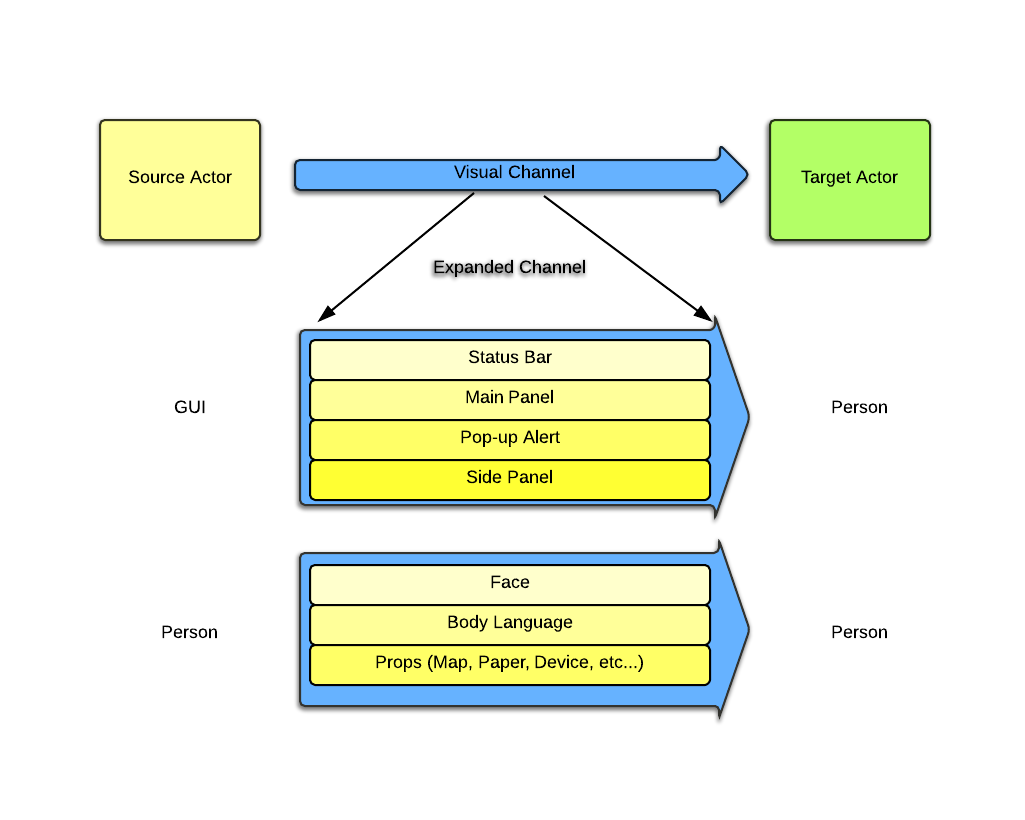
\includegraphics[width=5in]{layers.png}
\caption{Communication Channel Layers}
\label{fig:layers}
\end{center}
\end{figure}


\section{Metric Improvements}

In examining how to extract data from the simulation we came up with two approaches.  The first approach was to capture all of the raw data between each cycle and then construct metrics from these raw values such as the number of active channels, number of enabled transitions, total transition count, total output profile, etc�  After a brief examination of mounds of raw data it was determined that a better approach would be to simply collect specific data points that we cared about when they changed.  This made it easier to collect specific metrics, however, it created disjunct data sets which made it hard to compare the data in a time-line.  Also, as mentioned above, the metric dissemination was inconsistent.  This add-hoc approach to metric gathering also made it difficult to verify that the metrics being reported were accurate in relation to the other metrics.  Without clear accurate metrics it is impossible to realize the true value of the modeling framework we developed.  

To address these issues we used a mixed approach to gathering metrics.  See figure~\ref{fig:metric_gathering}  Each cycle the simulator asks the team for metrics, the team then asks each actor which then asks it�s sub-components.  This gives back all of the raw metric data contained in the simulation but as it is being passed back up the chain each component can perform calculations using the raw values it knows about to return specific metric values.  This maintains the timeline flow of the simulation and allows us to customize what metrics are actually calculated and displayed from the different levels.  An example of this is the Actor.  The Actor knows how many input channels he can listen on, his current state, etc�  The Actor does not directly know what transitions are enabled, how many inputs are in those transitions, etc..  Instead of trying to calculate all of this with multiple queries into the state the Actor simply asks the State object for its metrics.  The State then obtains/calculates metric values, obtaining metrics from sub-components if needed, before passing this values back to the Actor and eventually back to the simulator which displays the metrics to the user.  These metrics are shown in a  timeline paired with the Actor state.  The timeline itself represents each time a transition was fired, but more importantly it corresponds to the simultaneous state of each Actor, allowing the user to see which states have the highest workload and how an action by one Actor effects another.

\begin{figure}[h]
\begin{center}
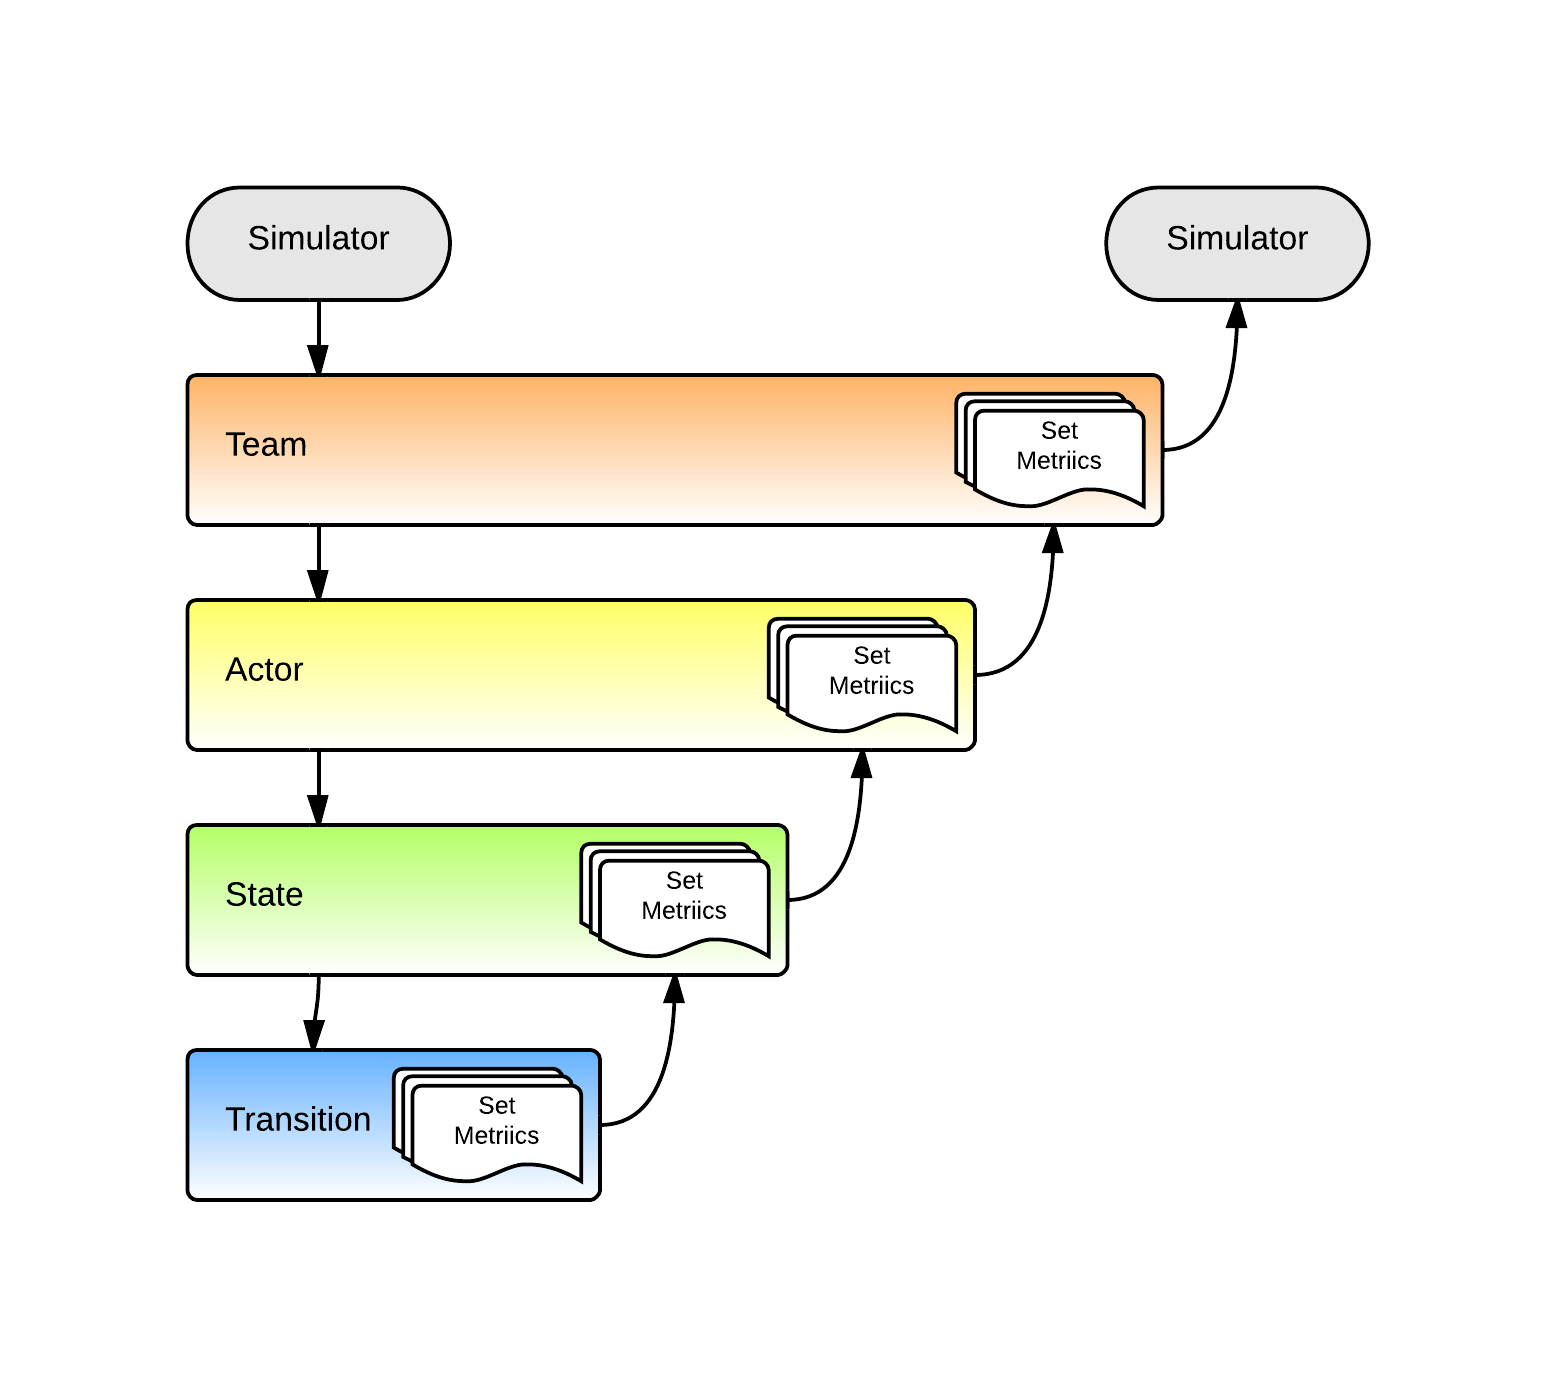
\includegraphics[width=6in]{metric_gathering.png}
\caption{Metric Gathering}
\label{fig:metric_gathering}
\end{center}
\end{figure}

\subsection{Wickens Workload Model}
	Gathering the raw values from the model was the easy part.  The harder part is to take these raw values and convert them into a value which reflects Actor workload.  Since our model relies on Wickens Multiple Resource Theory~\cite{wickens2002multiple}.  We decided to try and replicate the simple computational model for predicting workload presented with the theory.  Wickens computational model takes the task difficulty, ranging from 0 to 2 where 0 is automated and 2 is difficult, of two tasks and adds them together.  He then adds the number of dimensional conflicts between the tasks, max of 4, which gives a result between 0 and 8~\cite{wickens2002multiple}.
	The difficulty of applying this model to our metrics is that we have removed the concept of tasks and replaced it with the notion of state.  In order to replicate Wickens computational model we needed a way to represent task difficulty (resource demand) in a similar fashion.  We first looked at transition duration.  The longer a task takes the more difficult it is.  While this might work it prevents the modeler from placing an Actor into a long running simple task which we feel would degrade the usefulness of this framework.  Next we looked at resources.  The problem is that our modeling framework only tracks what resources are being used and when.  Good for finding conflicts but not for determining how much load those resources are under.  It is possible that Wickens ran into the same problem because his simple computational model relies on the modelers experience and intuition to set the task difficulty, which is likely more accurate than implicitly constructing task difficulty based on resource consumption.  This led to the realization that we had no good way of explicitly defining an Actors task difficulty.  To address this we defined a new term called Actor load.  
	
\subsection{Actor Load}
Actor load represents an abstraction of the load an Actor is under for any given state.  Similar to Wickens model we will use values from 0-4.  Each Actor state will define its own load.  A load of 0 represents little to no load on the actor.  These are automated or transitional states.  A load of 4 represents simultaneously performing multiple high difficulty tasks.  Any value between 1 and 3 is some combination of task difficulty and the number of tasks being performed.

\subsection{Applying Wickens Computational Model}
By placing Actor Load into the State portion of our models we can now replicate the simple computational model Wickens used in his measurements.  Using the State load as the task difficulty the next step is to find the dimensionality of the resource conflicts.  Since a state represents 1 or more tasks this also presents a challenge.  To best approximate Wickens model we needed metrics which could represent one or more tasks.  We accomplish this by making the assumption that if an Actor has input from multiple sources in a state then multiple tasks are being performed.  It should be noted that we check the input channels for each transition in the current state but only the outputs of the current transition.  With these assumptions we are now ready to calculate dimensional conflicts, Figure~\ref{fig:multipleresourcetheory}.
For the Stage dimension (perception, cognition, response) we check to see if there are multiple sources of input or multiple targets for output.  If there are then we increment the dimensionality.   
For the Modality dimension (Audio, Visual) we check if there are more than a single active channel, input or output, of type audio or visual.  If there is then we increment the dimensionality.  
For the Focus dimension we check if there is more than one source for tactile outputs, if there are then we increment the dimensionality.  We do not check inputs as we have no way of distinguishing if a visual channel has focus.  This may need to be addressed in future work. 
For the Codes dimension (Spacial, Verbal) we check that the total number of audio inputs and outputs is greater than 1 or that the total number of visual inputs, visual outputs, and tactile outputs is greater than 1.  If either value is greater than 1 then we increment the dimensionality.  

By adding the task difficulty (state load) and the dimensionality together we obtain an adapted Wickens metric which we can then compare with our own metrics.

\begin{figure}[h]
\begin{center}
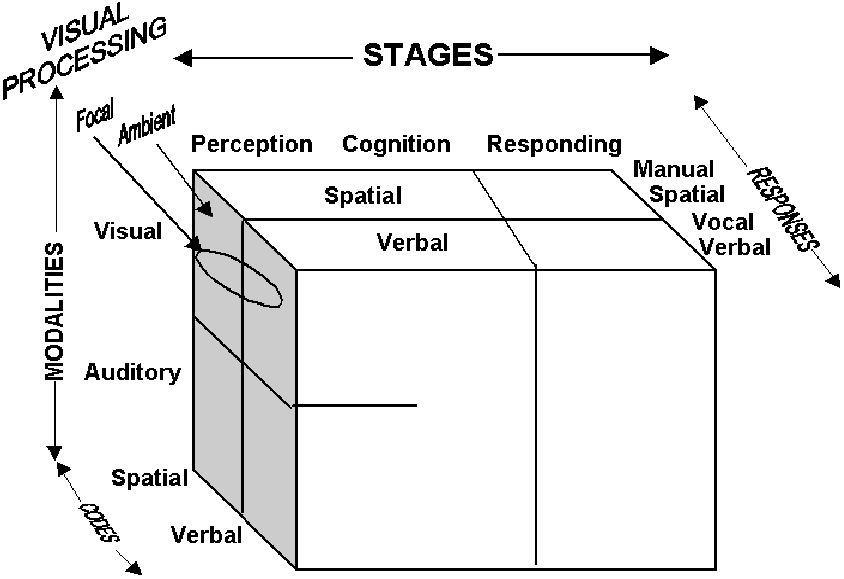
\includegraphics[width=6in]{multresourcetheory.png}
\caption{Multiple Resource Theory Dimensions}
\label{fig:multipleresourcetheory}
\end{center}
\end{figure}

\subsection{Changes to our Metrics}
For the resource workload category we now generate Actor metrics the following way.  Inputs are gathered from each transition that is part of the current state.  The outputs are collected from the active transition.  We also use the Actor load from the current state.  There are 2 main metrics the channel conflicts and the resource load.  Channel conflicts occur whenever more than one active channel share a type, such as multiple audio channels.  Since we currently only allow visual and audio input for human Actors this value ranges from 0 to 2.  The other metric is the resource load.  This metric attempts to quantify the load being placed on the Actors resources.  We break the resource load into two parts, input and output, the final result being the sum of both parts.  Each part is calculated by adding the number of active channels, number of layers read, number of memory objects read, and the number of active channel types.

For decision workload we have added input complexity and output complexity.  The input complexity is the total number of active inputs plus the number of memory inputs.  The output complexity is the number of output channels plus the number of memory outputs.  While there is overlap between these values and the resource workload metrics we leave it up to future work to analyze this relationship.  We have also modified the duration complexity metric.  Before adding Actor load we relied on the duration complexity to inform us of task difficulty.  We no longer apply the same weight to the durations.  Instead we are now using a logarithmic scale.  By assuming that durations are in seconds we classify any transition under a minute as 0 complexity and move up from there.  Our reasoning for this normalization is two fold.  First it is reasonable to assume that the more time a transition takes the more workload it requires, however, it is also reasonable to assume that there are diminishing returns associated with increasing the workload.  We would also like to compare the metrics together.  By normalizing this metric to a value between 0 and 6, for our model, we can show this metric side by side with the others.  


\subsection{Other Changes}
We also performed other refactorings to the modeling framework which facilitate the previously described changes and more.  As part of this re-factoring the connections to JPF were temporarily disabled in order to simplify the debugging process.  The results described in the next chapter were obtained by running the simulator as a stand alone application outside of JPF.  While this does prevent a deeper evaluation of the models state space the core model behavior still remains the same.  Unfortunately it prevented us from collecting the temporal workload metrics from the model.
